% set 0.5 inch indentation
\setlength{\parindent}{0.5in} 
% set paragraph space = 0 space
\setlength{\parskip}{0mm}
% set line space 1.5
\setlength{\baselineskip}{1.6em}

\chapter{INTRODUCTION} 

\section{Background of the Study}
Start your paragraph here; justified, 0.5” indentation. Maintain a 1.5 line spacing throughout. This section should consist of 2 pages maximum excluding figures and tables. This is NOT a Literature Review section.

Each paragraph should have at least 4 sentences. Paragraphs of more than 6 sentences should be split into two paragraphs. Follow the appropriate structure of writing a clear paragraph.  Consult your adviser about the subsections. Maintain one space between the last line of this section and the next subsection.

\section{Statement of the Problem}
Write approximately three paragraphs only. Each paragraph should have at least 4 sentences. Paragraphs of more than 6 sentences should be split into two paragraphs. Follow the appropriate structure of writing a clear paragraph.

\section{Research Questions- Discuss with your adviser.}
Introduce your research questions in one sentence followed by a bulleted list, left-aligned.

\begin{enumerate}
    \item Follow a 0.5” Tab setting
    \item
    \item
\end{enumerate}

\section{Objectives of the Study}
Introduce your main objective first in one sentence, followed by a bulleted list of specific objectives, left aligned.
\begin{itemize}
    \item Follow a 0.5” Tab setting
    \item
    \item
\end{itemize}

\section{Write the next section here.}
Start your paragraph here. 

\section{Organization of the Thesis}
Start your paragraph here. 


\begin{table}[ht]
  \caption[Random Table]{Random Table}
  \begin{center}
    \begin{tabular}{cccc}
      \hline \textbf{v1} & \textbf{v2} & \textbf{v3} & \textbf{Overall} \\ \hline
        78.67\% & 87.33\% & 94.92\% & 85.64\% \\ \hline
    \end{tabular}
  \end{center}
  \label{tab:random_table}
\end{table} 

\begin{table}[ht]
  \caption[Random Table 2]{Random Table 2}
  \begin{center}
    \begin{tabular}{cccc}
      \hline \textbf{v1} & \textbf{v2} & \textbf{v3} & \textbf{Overall} \\ \hline
        78.67\% & 87.33\% & 94.92\% & 85.64\% \\ \hline
    \end{tabular}
  \end{center}
  \label{tab:random_table_2}
\end{table} 

\begin{figure}[ht]
  \centering
  \caption[Random Figure]{Random Figure}
  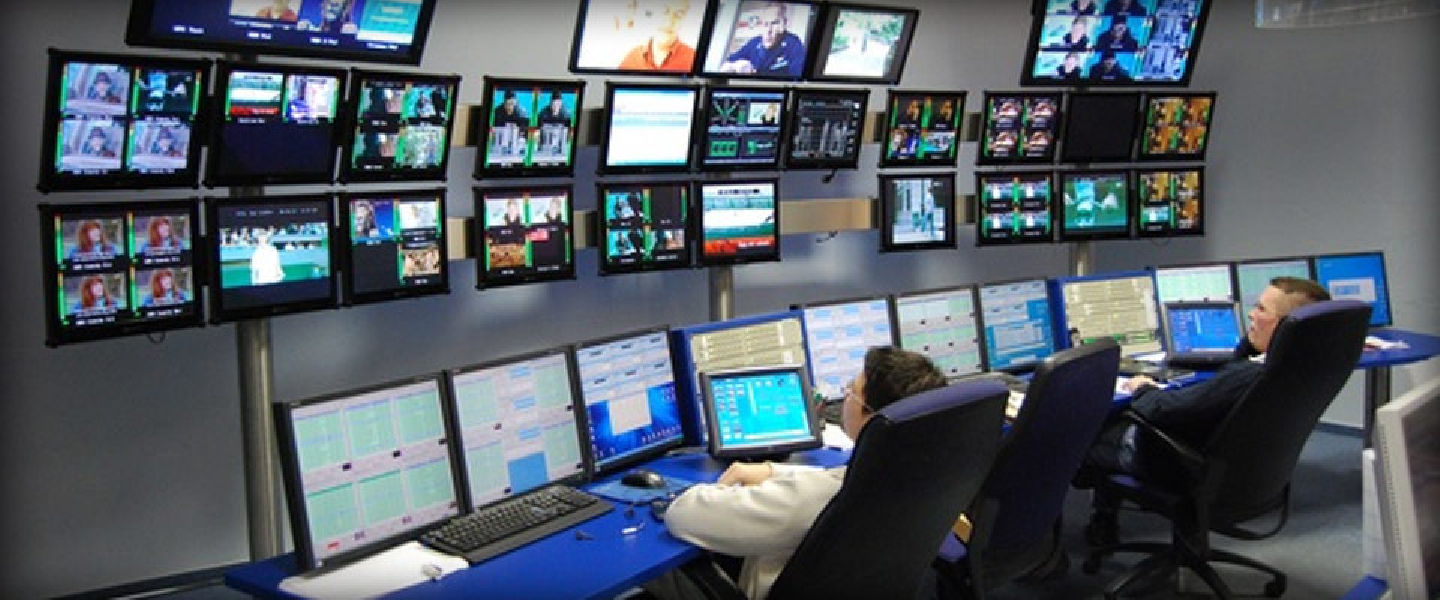
\includegraphics[width=0.75\textwidth]{figures/monitoring.pdf}
  \label{fig:random_figure}
\end{figure}